%Дата последнего изменения файла 26-05-2017
%\nonstopmode
\documentclass[12pt]{book}
%\usepackage[cp1251]{inputenc}
\usepackage{amsthm}
\usepackage{amsmath}
\usepackage{amssymb}
\usepackage{amsfonts}
\usepackage{mathtext}
\usepackage{mathrsfs}
\usepackage{cite}
\ifx\pdfoutput\undefined
\usepackage{graphicx}
\else
\usepackage[pdftex]{graphicx}
\fi

\usepackage{xypic}
\usepackage{epic}
%\usepackage{urwcyr}
%\usepackage{bng}
%\usepackage{pscyr}
%\usepackage[english,russian]{babel}
\usepackage[russian,english]{babel}
\usepackage[T2A]{fontenc}
\usepackage[utf8x]{inputenc}

\usepackage{multicol}
\premulticols=5pt \postmulticols=0mm \multicolsep=0mm
\usepackage{longtable}
%
%
%\usepackage{array}
%\usepackage{multirow}
%\renewcommand\multirowsetup{\centering}
%\usepackage{dcolumn}
\usepackage{graphicx}

% LAYOUT ----------------------------------------------------------
\usepackage{geometry}% Меняем поля страницы
\geometry{left=3.5cm}% левое поле
\geometry{right=1.5cm}% правое поле
\geometry{top=3cm}% верхнее поле
\geometry{bottom=2cm}% нижнее поле
\headsep=5mm%расстояние от верхнего колонтитула до текста
%
%Колонтитулы-----------------------------------------------------------
\usepackage{fancyhdr}%загрузим пакет
\pagestyle{fancy}%применим колонтитул
\fancyfoot{}\fancyhead{}% очистим футер (снизу) и хидер (сверху) на всякий случай
%\fancyhead[CE,CO]{\thepage}%номер страницы снизу по центру
\fancyfoot[LE,RO]{\thepage}%E - нечетные,  O - четные,  L - слева, R - справа, C - по центру
%\fancyhead[CO]{}%{текст-центр-нечетные}
%\fancyhead[LO]{Левый колонтитул}%
%\fancyhead[RE]{Правый колонтитул}%

%------------------------------------------------------------------

\makeatletter
\renewcommand{\@biblabel}[1]{#1.}

\renewcommand{\thesection}{\arabic{section}.}

\renewcommand{\section}{\@startsection
                                {section} %name
                                {1}       %level
                                {\z@}     %indent
                                {12pt}    %before skip
                                {10pt}    %after skip
                                {\reset@font\normalfont\bfseries\sffamily}}
                                          %font style

\newcommand{\titler}[1]{%
\vspace*{5mm}%

\noindent%
{\large\bf #1}%
\vspace*{5mm}%
}

\makeatother
\allowdisplaybreaks     % Разрешение переносить на другую страницу часть
                        % многострочной формулы
\sloppy                 %

\newcommand{\di}{\displaystyle}

%% аналог \- для внутритекстовых формул
%% пример: $y(x) \hm= R_\lambda f(x)
%% или : $Y(x)  \hm{:=} y_1(x) + y_2(x)
\newcommand{\hm}[1]{#1\nobreak\discretionary{}{\hbox{\ensuremath{#1}}}{}}
\relpenalty=10000 \binoppenalty=10000

%Обнулить все счетчики
\newcommand{\zerosetcounter}{
\setcounter{footnote}{0}\setcounter{section}{0}\setcounter{equation}{0}%
\setcounter{theorem}{0}\setcounter{lemma}{0}\setcounter{corollary}{0}\setcounter{prop}{0}
\setcounter{propos}{0}\setcounter{problem}{0}\setcounter{Theorem}{0}%
\setcounter{theoremnn}{0}\setcounter{lemmann}{0}\setcounter{corollarynn}{0}
\setcounter{propnn}{0}\setcounter{proposnn}{0}%
\setcounter{definitionn}{0}\setcounter{remarknn}{0}\setcounter{examplenn}{0}%
\setcounter{definition}{0}\setcounter{remark}{0}\setcounter{example}{0}%
\setcounter{hypothesis}{0}\setcounter{hypothesisnn}{0}\setcounter{theoremb}{0}
}

%%%%%%%%%%%%%%%%%%%%%%%%%%%%%%%%%%%%%%%%%%%%%%%%%%
%УДК
%%%%%%%%%%%%%%%%%%%%%%%%%%%%%%%%%%%%%%%%%%%%%%%%%%
\newcommand{\UDC}[1]{%
\vspace*{5mm}
\noindent\textsf{УДК %
#1}%
}

%%%%%%%%%%%%%%%%%%%%%%%%%%%%%%%%%%%%%%%%%%%%%%%%%%
%Заголовки статей
%%%%%%%%%%%%%%%%%%%%%%%%%%%%%%%%%%%%%%%%%%%%%%%%%%
\newcommand{\Rtitle}[1]{%
\begin{center}%
{ \bf\fontsize{14pt}{16pt}\sffamily%
#1}%
\end{center}%
}

\newcommand{\Etitle}[1]{%
\newpage
\begin{center}%
{ \bf\fontsize{12pt}{14pt}\sffamily%
#1}%
\end{center}%
}

%%%%%%%%%%%%%%%%%%%%%%%%%%%%%%%%%%%%%%%%%%%%%%%%%%%%%%%
%Авторы
%%%%%%%%%%%%%%%%%%%%%%%%%%%%%%%%%%%%%%%%%%%%%%%%%%%%%%%
\newcommand{\Rauthor}[1]{%
\centerline{%
\bf\fontsize{11pt}{14pt}
\sffamily%
#1}%
}

\newcommand{\Eauthor}[1]{%
\centerline{%
\bf\fontsize{11pt}{14pt}
\sffamily%
#1}%
}

%%%%%%%%%%%%%%%%%%%%%%%%%%%%%%%%%%%%%%%%%%%%%%%%%%%%%%%
%Сведения об авторах %affiliation
%%%%%%%%%%%%%%%%%%%%%%%%%%%%%%%%%%%%%%%%%%%%%%%%%%%%%%%
\newcommand{\Raffil}[1]{%
\begin{center}
\begin{minipage}{150mm}{%
\small\sffamily%
#1}%
\end{minipage}%
\end{center}
}

\newcommand{\Eaffil}[1]{%
\begin{center}%
\begin{minipage}{150mm}{%
\small\sffamily%
#1}%
\end{minipage}%
\end{center}
}

%%%%%%%%%%%%%%%%%%%%%%%%%%%%%%%%%%%%%%%%%%%%%%%%%%%%%%%
%E-mail
%%%%%%%%%%%%%%%%%%%%%%%%%%%%%%%%%%%%%%%%%%%%%%%%%%%%%%%
\newcommand{\Email}[1]{%
\vspace*{-3mm}
\centerline{%
\small\textit{%
E-mail: #1}}%
\vspace*{3mm}%
}

%%%%%%%%%%%%%%%%%%%%%%%%%%%%%%%%%%%%%%%%%%%%%%%%%%%%%
%Аннотация
%%%%%%%%%%%%%%%%%%%%%%%%%%%%%%%%%%%%%%%%%%%%%%%%%%%%%
\newcommand{\Rabstract}[1]{%
\centerline{%
\begin{minipage}{150mm}%
{%\setlength{\parindent}{4mm}
\small\sffamily%
#1}%
\end{minipage}}%
}

\newcommand{\Eabstract}[1]{%
\centerline{%
\begin{minipage}{150mm}%
{%\setlength{\parindent}{4mm}
\small\sffamily%
#1}%
\end{minipage}}%
}

%%%%%%%%%%%%%%%%%%%%%%%%%%%%%%%%%%%%%%%%%%%%%%%%%%%%%
%Ключевые слова
%%%%%%%%%%%%%%%%%%%%%%%%%%%%%%%%%%%%%%%%%%%%%%%%%%%%%
\newcommand{\Rkeywords}[1]{%
\vspace*{3mm}%
\centerline{%
\begin{minipage}{150mm}%
{%\setlength{\parindent}{4mm}
\small\sffamily%
\textit{Ключевые слова:} #1.}%
\end{minipage}}%
\vspace*{3mm}%
}

\newcommand{\Ekeywords}[1]{%
\vspace*{3mm}%
\centerline{%
\begin{minipage}{150mm}%
{%\setlength{\parindent}{4mm}
\small\sffamily%
\textit{Key words:} #1.}%
\end{minipage}}%
\vspace*{3mm}%
}

\newlength{\realparindent}%


%%%%%%%%%%%%%%%%%%%%%%%%%%%%%%%%%%%%%%%%%%%%%%%%%%%%%
%Библиографический список
%%%%%%%%%%%%%%%%%%%%%%%%%%%%%%%%%%%%%%%%%%%%%%%%%%%%%
\makeatletter
\renewcommand{\chapter}{\@startsection{chapter}{1}{0em}%
{3.5ex plus 1ex minus .2ex}{.9ex plus.2ex}%
{\zerosetcounter}}
%Стили нумерации формул, списка литературы
\addto\captionsrussian{%
\def\bibname{}%Меняем заголовок литературы
}%
\renewcommand{\@biblabel}[1]{#1.}%Оформление номера в списке литературы
\makeatother

\newenvironment{Rtwocolbib}
{%
\vspace*{3mm} %
\noindent
{\normalfont\bfseries\sffamily Библиографический список}%
\def\bibname{}
\small
%\begin{multicols}{2}%
\vspace*{-12mm}%
\begin{thebibliography}{99}
\setlength{\itemsep}{-4pt}
}{%
\end{thebibliography}
%\end{multicols}%
\normalsize}%

\newenvironment{Etwocolbib}
{%
\vspace*{1mm} %
\noindent
{\normalfont\bfseries\sffamily References}%
%\begin{otherlanguage}{english}
\small
%\begin{multicols}{2}%
%\vspace*{-45pt}%
\begin{enumerate}
\setlength{\itemsep}{-4pt}
}{%
\end{enumerate}
%\end{multicols}%
%\end{otherlanguage}
\normalsize
}%
%%%%%%%%%%%%%%%%%%%%%%%%%%%%%%%%%%%%%%%%%%%%%%%%%%%%%%%%%%%
\renewcommand{\arraystretch}{1.1}

%%%%%%%%%%%%%%%%%%%%%%%%%%%%%%%%%%%%%%%
%Благодарности
%%%%%%%%%%%%%%%%%%%%%%%%%%%%%%%%%%%%%%%
\renewcommand{\thanks}[1]{%
\vspace*{3mm}%
\noindent\textit{Благодарности. #1.}%
\vspace{2mm}%
}%

\newcommand{\ethanks}[1]{%
%\vspace*{3mm}%
\small
\noindent\textit{Acknowledgements: #1.}%
\vspace{3mm}%
\normalsize
}%

%-------------------------------------------------
\theoremstyle{plain}
%Нумерованные
\newtheorem{theorem}{\indent Теорема}
\newtheorem{lemma}{\indent Лемма}
\newtheorem{corollary}{\indent Следствие}
\newtheorem{prop}{\indent Утверждение}
\newtheorem{propos}{\indent Предложение}
\newtheorem{problem}{\indent Задача}
\newtheorem{Theorem}{\indent Theorem}
\newtheorem{hypothesis}{\indent Предположение}
\newtheorem{Etheorem}{\indent Theorem}
\newtheorem{Eproposition}{\indent Proposition}
\newtheorem{Corollary}{\indent Corollary}
\newtheorem{Lemma}{\indent Lemma}
\newtheorem{theoremb}{\indent Теорема}
\renewcommand{\thetheoremb}{\Alph{theoremb}}%Нумерация теорем A, B, C
\usepackage[labelformat=empty]{caption}
\usepackage{graphicx}
\renewcommand{\Pr}{{\mathbf P}}

\theoremstyle{remark}
\newtheorem{Example}{\indent Example}


%Двойная нумерация
\newtheorem{theoremnn}{\indent Теорема}[section]
\newtheorem{lemmann}{\indent Лемма}[section]
\newtheorem{corollarynn}{\indent Следствие}[section]
\newtheorem{propnn}{\indent Утверждение}[section]
\newtheorem{proposnn}{\indent Предложение}[section]
\newtheorem{hypothesisnn}{\indent Предположение}[section]

\theoremstyle{plain}
%Ненумерованные окружения
\newtheorem*{theorem*}{\indent Теорема}%Просто теорема (без номера)
\newtheorem*{lemma*}{\indent Лемма}
\newtheorem*{corollary*}{\indent Следствие}
\newtheorem*{Corollary*}{\indent Corollary}
\newtheorem*{prop*}{\indent Утверждение}
\newtheorem*{propos*}{\indent Предложение}
\newtheorem*{hypothesis*}{\indent Предположение}
%-------------------------------------------------
\theoremstyle{definition}
\newtheorem{definitionn}{\indent Определение}[section]
\newtheorem{remarknn}{\indent Замечание}[section]
\newtheorem{examplenn}{\indent Пример}[section]

\newtheorem{definition}{\indent Определение}
\newtheorem{remark}{\indent Замечание}
\newtheorem{example}{\indent Пример}
\newtheorem{Remark}{\indent Remark}
\newtheorem{Question}{\indent Question}
\newtheorem{Definition}{\indent Definition}

\newtheorem*{definition*}{\indent Определение}
\newtheorem*{remark*}{\indent Замечание}
\newtheorem*{example*}{\indent Пример}

\renewenvironment{proof}{\indent\textbf{Доказательство. }}{\hfill$\Box$}

\newcommand{\const}{\mathrm{const}}
\newcommand{\Span}{\mathrm{Span}\,}
\renewcommand{\Re}{\,\mathrm{Re}\,}
\renewcommand{\Im}{\,\mathrm{Im}\,}
\newcommand{\sgn}{\mathrm{sgn}\,}
\newcommand{\diag}{\mathrm{diag}\,}
%\numberwithin{equation}{section}%Двойная нумерация формул
%Если Вы подключаете новый пакет, то обязательно сообщите об этом в комментариях к тексту статьи.
\begin{document}
%%%%%%%%%%%%%%%%%%%%%%%%%%%%%%%%%%%%%%%%%%%%%%%%%%%%%%%%%%%%%%%%%%%%
\fancyhead[CE]{МАТЕМАТИКА}%Раздел журнала
\fancyhead[CO]{В.М.~Кочеганов. Классификация состояний марковской цепи в модели тандема с циклическим управлением с продлением}%

    \UDC{519.248}

\Rtitle{КЛАССИФИКАЦИЯ СОСТОЯНИЙ МАРКОВСКОЙ ЦЕПИ В МОДЕЛИ ТАНДЕМА С ЦИКЛИЧЕСКИМ УПРАВЛЕНИЕМ С ПРОДЛЕНИЕМ}%

%\thispagestyle{izsc}%не убирать!!!
\Rauthor{В.~М.~Кочеганов}%

%Фамилия Имя отчество, ученая степень, должность (с указанием кафедры, отдела), место работы (полное
%официальное название учреждения, почтовый адрес), e-mail;
\Raffil{Кочеганов Виктор Михайлович, аспирант кафедры программной инженерии, национальный исследовательский Нижегородский государственный университет
{им.Н.И.Лобачевского}, 603950, Россия, Н.Новгород, пр.~Гагарина, 23, kocheganov@gmail.com}


\Rabstract{На данный момент существует ограниченное число работ, посвященных тандемам перекрестков. В литературе, как правило, изучаются следующие виды алгоритмов управления: циклический алгоритм с фиксированной длительностью, циклический алгоритм с петлей, циклический алгоритм со сменой режимов и т.д. При построении математических моделей сетей массового обслуживания и тандемов в частности, как правило, применяется описательный подход. При таком подходе задание входных потоков и алгоритмов обслуживания производится на содержательном уровне, законы распределения длительностей обслуживания требований считаются известными и задаются с помощью интегральной функции распределения времени обслуживания произвольного требования. При этом не удается решить проблему изучения выходящих потоков из узлов, а также рассмотреть сети с немгновенным перемещением требований между узлами и с зависимыми, разнораспределенными длительностями обслуживания требований.
В настоящей работе применяется новый подход к построению вероятностных моделей тандемов конфликтных систем массового обслуживания с различными алгоритмами управления в узлах. В рамках этого подхода удается решить проблему выбора описаний $\omega$ элементарных исходов случайного эксперимента и математически корректно определить случайный процесс, описывающий эволюцию рассматриваемой системы, а также решить перечисленные выше частные задачи. На основе конструктивно заданного вероятностного пространства удается строго обосновать достижимость одних состояних из других, тем самым полностью описав единственный класс существенных состояний марковской цепи, описывающей динамику тандема.}\Rkeywords{стационарное распределение, управляющая система массового обслуживания, циклический алгоритм с продлением, конфликтные потоки, многомерная счетная марковская цепь, существенные состояния}

%%%%%%%%%%%%%%%%%%%%%%%%%%%%%%%%%%%%%%%%%%%%%%%
%Текст статьи
%%%%%%%%%%%%%%%%%%%%%%%%%%%%%%%%%%%%%%%%%%%%%%%


\section{ПОСТАНОВКА ЗАДАЧИ И МАТЕМАТИЧЕСКАЯ МОДЕЛЬ}\label{ProblemStatement}
В работах~\cite{Haight:1963}~--~\cite{Yamada} представлены различные модели тандемов управляющих систем обслуживания в постановке задач автомобильного трафика. Исходной задачей для исследования в настоящей работе яляется анализ тандема двух последовательных перекрестков, автомобили между которыми перемещаются немгновенно, и обслуживание на одном из перекрестков допускает продление. Формулируя задачу в терминах управляющих систем обслуживания, будем предполагать, что в  первой системе тандема обслуживаются конфликтные потоки по циклическому алгоритму, а во второй --- по алгоритму с продлением. Данная тандемная сеть
подробно описана в работах~\cite{Kocheganov:2017:1, Kocheganov:2018}. Развиваемый там подход позволил представить
тандем систем как единую систему массового обслуживания. Напомним существенные
моменты из описания системы.  На вход обслуживающему устройству поступают четыре
входных потока требований: $\Pi_1$, $\Pi_2$, $\Pi_3$ и $\Pi_4$.  Требования
входного потока~$\Pi_j$ поступают в очередь $O_j$ с неограниченной вместимостью,
$j \in \{1,2,3,4\}$. Требования из очереди $O_j$ обслуживаются в порядке
поступления. Требования входных потоков~$\Pi_1$ и~$\Pi_3$ формируются внешней
средой, имеющей всего одно состояние. Каждый из этих потоков является
неординарным пуассоновским потоком. Обозначим $\lambda_1$ и $\lambda_3$
интенсивности потоков групп требований потоков $\Pi_1$ и $\Pi_3$
соответственно. Производящая функция количества требований в группе по потоку
$\Pi_j$ имеет вид $f_j(z) = \sum_{\nu=1}^{\infty} p_{\nu}^{(j)} z ^{\nu}$, $j\in
\{1,3\}$.  Предполагается, что $f_j(z)$ сходится для любого $z\in \mathbb{C}$
такого, что $|z|<\nobreak\discretionary{}{\hbox{$\mathsurround=0pt
    <$}}{}(1+\varepsilon)$, $\varepsilon>0$. После обслуживания требования из
очереди $O_1$ поступают обратно в систему как требования потока
$\Pi_4$. Требования потока~$\Pi_4$, в свою очередь, после обслуживания поступают
в систему в качестве требований потока $\Pi_2$. Потоки $\Pi_2$ и $\Pi_3$
конфликтные в том смысле, что их требования не могут быть обслужены
одновременно. 

Зафиксируем положительные целые числа $d$, $n_0$, $n_1$, $\ldots$,
$n_d$. Тогда множество состояний обслуживающего устройства будет выглядить следующим образом: $\Gamma=\{\Gamma^{(k,r)} \colon k=0,1,\ldots,d; r=1,2,\ldots
n_k\}$. В состоянии  $\Gamma^{(k,r)}$ сервер находится в течение неслучайного
времени  $T^{(k,r)}$. Алгоритм смены состояний учитывает как предыдущее
состояние прибора, так и длину очереди $O_3$ в момент принятия решения и
формально описан в работе~\cite{Kocheganov:2017:1}. 

Для задания процесса обслуживания используются потоки насыщения
$\Pi^{\mathrm{\text{нас}}}_1$, $\Pi^{\mathrm{\text{нас}}}_2$, $\Pi^{\mathrm{\text{нас}}}_3$,
$\Pi^{\mathrm{\text{нас}}}_4$.  Число требований в потоке насыщения
$\Pi^{\mathrm{\text{нас}}}_j$ за время $T^{(k,r)}$ неслучайно и равно $\ell(k,r,j)$, если
обслуживающее устройство находится в состоянии $\Gamma^{(k,r)}\in \Gamma$.

Представленная система массового обслуживания может рассматриваться как
кибернетическая управляющая система.  Схема управляющей системы
представлена на Рис.~1. На схеме присутствуют следующие блоки: внешняя среда с
одним состоянием, входные полюса (входные потоки $\Pi_1$, $\Pi_2$, $\Pi_3$,
$\Pi_4$ и потоки насыщения $\Pi^{\mathrm{\text{нас}}}_1$, $\Pi^{\mathrm{\text{нас}}}_2$, $\Pi^{\mathrm{\text{нас}}}_3$,
$\Pi^{\mathrm{\text{нас}}}_4$), внешняя память (очереди $O_1$, $O_2$, $O_3$, $O_4$), устройство по
переработке внешней памяти (устройства поддержания дисциплин очередей
$\delta_1$, $\delta_2$, $\delta_3$, $\delta_4$), внутренняя память (обслуживающее
устройство, ОУ), устройство по переработке внутренней памяти (граф переходов из
одного состояния ОУ в другое), выходные полюса (выходные потоки
$\Pi^{\mathrm{\text{вых}}}_1$, $\Pi^{\mathrm{\text{вых}}}_2$,
$\Pi^{\mathrm{\text{вых}}}_3$, $\Pi^{\mathrm{\text{вых}}}_4$).
\sloppy 

\begin{figure}[h!]
   \centering
    \includegraphics[width=17cm]{SystemScheme.eps}
    \caption {Рис.~1: Схема СМО как управляющей кибернетической системы ({Queuing system as cybernetic system scheme})}
\end{figure}

В работе~[2] были выделены информация, координаты и функция данной системы. Это
позволило конструктивно задать последовательности случайных величин и случайных
элементов, описывающих дискретную временную шкалу наблюдения и состояния всех
блоков схемы. В частности, в качестве дискретной временной шкалы выбрана
последовательность $\tau_0=0$, $\tau_1$, $\tau_2$, $\ldots$ моментов смены
состояния обслуживающего устройства. Обозначим $\Gamma_i\in\Gamma$, $i=1$, $2$,
\ldots{}, состояние обслуживающего устройства в течение времени
$\left(\tau_{i-1};\tau_i\right]$ и $\Gamma_0\in \Gamma$~--- его состояние в момент
времени $\tau_0$, и пусть $\varkappa_{j,i} \in \mathbb{Z}_+ $~--- количество
требований в очереди $O_j$ в момент времени $\tau_i$, , $i\geqslant 0$.  
Было доказано, что стохастическая последовательность $\{(\Gamma_i,
\varkappa_{1,i}, \varkappa_{2,i}, \varkappa_{3,i}, \varkappa_{4,i}); i=0, 1,
\ldots\}$ является однородной цепью Маркова.
%Свойства последовательности $\{(\Gamma_i,\varkappa_{3,i}); i \geqslant 0\}$ изучены в работах~[1,3].

\section{КЛАССИФИКАЦИЯ СОСТОЯНИЙ МАРКОВСКОЙ ЦЕПИ $\boldsymbol{\{(\Gamma_i,
\varkappa_{i}); i=0, 1,
\ldots\}}$ }\label{Classification}
Теперь поставим вопрос о существенных состояниях марковской цепи 
$$\{(\Gamma_i,
\varkappa_{i}); i=0, 1,
\ldots\},$$
которая описывает динамику исследуемой в работе кибернетической системы. Мы последовательно рассмотрим состояния разного вида и определим сообщающиеся подклассы. 
На первом этапе выясним,  что состояния вида 
$$(\Gamma^{(0,  \tilde{r})},  \tilde{x}),  \quad \tilde{r} = \overline{1,  n_0},  \tilde{x}=(0,  0,  L+1,  0), $$ 
являются существенными (леммы \ref{classification:arithm:1},  \ref{classification:arithm:2},  \ref{first:lemma}). Лемма~\ref{classification:arithm:1},  в частности,  говорит о том,  что из состояний продления с произвольным количеством требований в очередях $O_1$,  $O_2$ и $O_4$ можно перейти с ненулевой вероятностью также в состояние продления,  но с пустыми очередями $O_1$,  $O_2$ и $O_4$.


\begin{lemma}\label{classification:arithm:1}
Состояния вида 
$$(\Gamma^{(0,  \tilde{r})}, (0,  0,  \tilde{x}_3,  0)),  \quad \tilde{r} = \overline{1,  n_0},  \tilde{x}_3 \geqslant x_{3,  0}, $$
достижимы из состояний вида 
$$(\Gamma^{(0,  r_0)},  x^0),  \quad r_0=\overline{1,  n_0},  x^0 \hm\in \mathbb{Z}_+^4,  x^0\hm=(x_{1, 0},  x_{2, 0},  x_{3, 0},  x_{4, 0}),  x_{3,  0} \leqslant L.$$
\end{lemma}
\begin{proof}
Доказательство состоит из нескольких этапов. Сначала, основываясь на заложенных в построенное вероятностное пространство свойствах, доказывается,  что вероятность каждого шага в цепочке
\begin{equation*}
(\Gamma^{(0, r_0)}, x^0) \rightarrow (\Gamma^{(0, r_0\oplus_{0}1)}, x^1) \rightarrow (\Gamma^{(0, r_0\oplus_{0}2)},  x^2) \rightarrow \ldots \rightarrow (\Gamma^{(0,  r_0\oplus_{0} N_2)},  x^{N_2})
\end{equation*}
для любого $N_2 > 0$ положительна. Вектора $x^j$,  $j>1$,  определим ниже.

Пусть система стартовала в состоянии $(\Gamma_{0},  \varkappa_{0}) = (\Gamma^{(0, r_0)},  x^0)$.
Из построения следует, что 
\begin{equation*}
\Gamma_1 = h(\Gamma_0, \varkappa_{3, 0}) = h(\Gamma^{(0, r_0)},  x_{3, 0}) = \Gamma^{(0, r_0\oplus_{0}1)},
\end{equation*}
где отображение $h(\cdot,\cdot)$ определено в работе~\cite{Kocheganov:2018}.

Положим
\begin{multline*}
x^1 =(x_{1, 1}, x_{2, 1}, x_{3, 1}, x_{4, 1}) =\left(\max{\{0,  x_{1, 0} - \ell(0, r_0\oplus_{0}1, 1)\}}; \right. \\
\left. \max{\{0,  x_{2, 0} + x_{4, 0}  - \ell(0, r_0\oplus_{0}1, 2)\}}; x_{3, 0};\min{\{x_{1, 0}, \ell(0, r_0\oplus_{0}1, 1)\}}\right).
\end{multline*}
В общем случае
\begin{equation*}
\Pr (\{\omega\colon\Gamma_{j+1}=\Gamma^{(0,  r_0\oplus_{0}j+1)}, \varkappa_{j+1}=x^{j+1} \} |\{\omega\colon \Gamma_{j}=\Gamma^{(0,  r_0\oplus_{0}j)},  \varkappa_j=x^j\}) > 0 
\end{equation*}
для 
\begin{multline*}
x^{j+1}  =\left(\max{\{0,  x_{1,  j} - \ell(0,  r_0\oplus_{0}j+1,  1)\}}; \right. \\
\left. \max{\{0,  x_{2, j} + x_{4, j}  - \ell(0,  r_0\oplus_{0}j+1,  2)\}}; x_{3,  0};\min{\{x_{1,  j},  \ell(0,  r_0\oplus_{0}j+1,  1)\}}\right), 
\end{multline*}
где $j = 1$,  $2$,  $\ldots$,  $N_2$. Число $N_2$ будет определено ниже.

Для некоторого $N_1>0$ количества требований $x_{1,  N_1}$,  $x_{2,  N_1}$ и $x_{4,  N_1}$ в соответствующих очередях $O_1$,  $O_2$ и $O_4$ рано или поздно станут равными нулю,  т.е. 
\begin{equation*}
\Pr (\{\omega\colon\Gamma_{N_1}=\Gamma^{(0,  r_0\oplus_{0}N_1)}, \varkappa_{N_1}=x^{N_1} \}| \{\omega\colon\Gamma_{N_1-1}=\Gamma^{(0,  r_0\oplus_{0}(N_1-1))},  \varkappa_{N_1-1}=x^{N_1-1}\}) > 0, 
\end{equation*}
для $x^{N_1} = \left(0; 0; x_{3,  0};0\right)$. Поскольку все состояния продления образуют цикл (а только такие графы переходов рассматриваются в работе),  то существует такое число $N_2>N_1$,  что $r_0 \oplus_0  N_2 = \tilde{r} \ominus_0 1$ и 
\begin{equation*}
\Pr (\{\omega\colon\Gamma_{N_2}=\Gamma^{(0,  r_0\oplus_{0} N_2)}, \varkappa_{N_2}=x^{N_2} \}|\\ \{\omega\colon\Gamma_{N_2-1}=\Gamma^{(0,  r_0\oplus_{0}(N_2-1))}, \varkappa_{N_2-1}=x^{N_2-1}\}) > 0, 
\end{equation*}
где $x^{N_2} = (0, 0, x_{3, 0}, 0)$.
Для завершения доказательства теперь необходимо рассмотреть переход
\begin{equation*}
 (\Gamma^{(0,  r_0\oplus_{0} N_2)},  x^{N_2})  \rightarrow (\Gamma^{(0,  \tilde{r})},  x^{N_2+1}), 
\end{equation*}
то есть оценить вероятность 
\begin{equation*}
\Pr (\{\omega\colon\Gamma_{N_2+1}=\Gamma^{(0,  \tilde{r})},  \varkappa_{N_2+1}= x^{N_2+1} \}| \{\omega\colon\Gamma_{N_2}=\Gamma^{(0,  r_0\oplus_{0}N_2)},  \varkappa_{N_2}=x^{N_2}\}), 
\end{equation*}
где 
$$(\Gamma_{N_2+1},  \varkappa_{N_2+1})= (\Gamma^{(0,  r_0\oplus_{0} N_2))},  x^{N_2+1}) = (\Gamma^{(0,  \tilde{r})} ,  (0,  0,  \tilde{x}_3,  0) )$$
есть конечное состояние.

Положим $N = N_2+1$ и соберем все воедино:
\begin{multline*}
\Pr(\{\omega\colon\Gamma_{N}=\Gamma^{(0,  \tilde{r} )},  \varkappa_{N}=x^N\}| \{\omega\colon
\Gamma_{0}=\Gamma^{(0,  r_0)},  \varkappa_{0}=x^0\}) = \\ =
\Pr(\{\omega\colon\Gamma_{N_2+1}=\Gamma^{(0,  \tilde{r} )},  \varkappa_{ N_2+1}=x^{N_2+1}\}|\{\omega\colon
\Gamma_{0}=\Gamma^{(0,  r_0)},  \varkappa_{0}=x^0\}) \geqslant \\ 
\geqslant
\Pr(C|\{\omega\colon\Gamma_{0}=\Gamma^{(0,  r_0)},  \varkappa_{0}=x^0\}), 
\end{multline*}
где 
\begin{multline*}
    C =\left\{\omega\colon\Gamma_{ N_2+1}=\Gamma^{(0,  \tilde{r} )},  \varkappa_{ N_2+1}=x^{N_2+1}\right\} \cap \left\{ \omega\colon \Gamma_{ N_2}=\Gamma^{(0,  \tilde{r} \ominus_0 1 )},  \varkappa_{N_2}=x^{N_2}\right\} \cap\ldots \Bigr.\\ \Bigl.
\ldots \cap \left\{\omega\colon\Gamma_{2}=\Gamma^{(0,  r_0\oplus_{0}2)}, \varkappa_{2}=x^2\right\} \cap \left\{\omega\colon \Gamma_{1}=\Gamma^{(0,  r_0\oplus_{0}1)}, \varkappa_{1}=x^1\right\}.
\end{multline*}
Наконец,  из теоремы умножения и марковского свойства заключаем,  что 
\begin{multline*}
\Pr\Bigl(\Bigl\{\omega\colon \Gamma_{N}=\Gamma^{(0, \tilde{r} )},  \varkappa_{N}=x^N\Bigr\} \,  \Big|\Bigl\{\omega\colon 
\Gamma_{0}=\Gamma^{(0,  r_0)},  \varkappa_{0}=x^0\Bigr\}\Bigr) \geqslant \\ 
\geqslant
\Pr\Bigl(\Bigl\{\omega\colon \Gamma_{N_2+1}=\Gamma^{(0,  \tilde{r} )},  \varkappa_{ N_2+1}=x^{N_2+1}\Bigr\}\,  \Big| \Bigl\{\omega\colon \Gamma_{ N_2}=\Gamma^{(0,  \tilde{r} \ominus_0 1 )},  \varkappa_{N_2}=x^{N_2}\Bigr\}\Bigr) \times 
%
\\ \times
\Pr\Bigl(\!\Bigl\{\omega\colon\Gamma_{ N_2}=\Gamma^{(0,  \tilde{r} \ominus_0 1 )},  \varkappa_{N_2}=x^{N_2}\Bigr\} \, \Big| \Bigl\{\omega\colon \Gamma_{ N_2-1}=\Gamma^{(0, \tilde{r} \ominus_0 2 )},  \varkappa_{N_2-1}=x^{N_2-1}\Bigr\}\Bigr) \times 
%
\\ \times \ldots
\times 
\Pr\Bigl(\Bigl\{\omega\colon\Gamma_{2}=\Gamma^{(0,  r_0\oplus_{0}2)}, \varkappa_{2}=x^2\Bigr\}\,  \Big|  \Bigl\{\omega\colon \Gamma_{1}=\Gamma^{(0,  r_0\oplus_{0}1)},  \varkappa_{1}=x^1\Bigr\}\Bigr) \times 
\\
\times
\Pr\Bigl(\Bigl\{\omega\colon\Gamma_{1}=\Gamma^{(0,  r_0\oplus_{0}1)},  \varkappa_{1}=x^1\Bigr\} \, \Big| \Bigl\{\omega\colon \Gamma_{0}=\Gamma^{(0,  r_0)},  \varkappa_{0}=x^0\Bigr\}\Bigr)>0, 
\end{multline*}
что и требовалось доказать. Таким образом,  каждый переход в цепочке переходов
\begin{multline*}
(\Gamma^{(0, r_0)}, x^0) \rightarrow (\Gamma^{(0, r_0\oplus_{0}1)}, x^1) \rightarrow (\Gamma^{(0, r_0\oplus_{0}2)},  x^2) \rightarrow \ldots \\ \ldots \rightarrow (\Gamma^{(0,  r_0\oplus_{0} N_2)},  x^{N_2})   \rightarrow (\Gamma^{(0,  \tilde{r})},  x^{N_2+1})
\end{multline*}
от начального до конечного состояний имеет ненулевую вероятность.
\end{proof}

Дальнейшие результаты приведем без доказательства.

В лемме~\ref{classification:arithm:2} показано,  как из произвольного состояния цикла $k_0 > 0$ перейти в состояние продления с заданным количеством требований $0$,  $0$,  $L+1$,  $0$  в очередях $O_1$,  $O_2$,  $O_3$,  $O_4$ соответственно.
\begin{lemma}\label{classification:arithm:2}
Состояния вида 
$$(\Gamma^{(0,  \tilde{r})},  \tilde{x}),  \quad \tilde{r} = \overline{1,  n_0},  \tilde{x}=(0,  0,  L+1,  0), $$
 достижимы из состояний вида 
 \begin{equation*}
 (\Gamma^{(k_0,  r_0)},  x^0),  \quad k_0 > 0,  r_0=\overline{1,  n_{k_0}},  x^0 \in \mathbb{Z}_+^4.
 \end{equation*}
\end{lemma}
Лемма~\ref{first:lemma} заключает о том,  что состояния вида $(\Gamma^{(0, \tilde{r})}, (0, 0, L+1, 0) )$ являются существенными. Наличие некоторого множества существенных состояний позволит в дальнейшем найти все оставшиеся существенные состояния.
\begin{lemma}\label{first:lemma}
Состояния вида 
$$(\Gamma^{(0,  \tilde{r})},  \tilde{x}),  \quad \tilde{r} = \overline{1,  n_0},  \tilde{x}=(0,  0,  L+1,  0), $$
достижимы из любых состояний системы,  то есть из состояний вида 
 $$(\Gamma^{(k_0,  r_0)},  x^0),  \quad k_0=\overline{0,  d},  r_0=\overline{1,  n_{k_0}},  x^0 \in \mathbb{Z}_+^4.$$
Таким образом,  состояния $(\Gamma^{(0,  \tilde{r})},  \tilde{x})$ являются существенными.
\end{lemma}



В леммах \ref{classification:arithm:3},  \ref{classification:arithm:4},  \ref{classification:arithm:5} определяются состояния,  сообщающиеся с существенными состояниями $(\Gamma^{(0,  r_0)},  x^0)$,  $x_0=(0,  0,  L+1,  0)$,  $r_0=\overline{1,  n_0}$. Таким способом определится все множество существенных состояний. В частности,  лемма \ref{classification:arithm:3} касается состояний циклов.
\begin{lemma}\label{classification:arithm:3}
Состояния вида 
\begin{align*}
    (\Gamma^{(\tilde{k},  \tilde{r})},  \tilde{x}),  \quad
&\tilde{x}=(0,  0,  \tilde{x}_3,  0),  \tilde{x}_3\geqslant\max{\{0,  L+1-\sum_{s=1}^{\tilde{r}} \ell(\tilde{k},  s,  3)\}},  \\ &\tilde{r} = \overline{1,  n_{\tilde{k}}},  \tilde{k}>0,  \Gamma^{(\tilde{k},  1)}=h_3(r_0), 
\end{align*}
 достижимы из состояний вида
 $$(\Gamma^{(0,  r_0)},  x^0),  \quad x_0=(0,  0,  L+1,  0),  r_0=\overline{1,  n_0}.$$
\end{lemma}

\begin{lemma}\label{classification:arithm:4}
Состояния вида 
\begin{equation*}
    (\Gamma^{(0,  \tilde{r})},  \tilde{x}),  \quad 
\tilde{x}=(0,  0,  \tilde{x}_3, 0),  \tilde{x}_3 \geqslant \max{\{0,  L+1-\sum_{s=1}^{n_{\tilde{k}}} \ell(\tilde{k},  s,  3)\}}, 
\end{equation*}
где $\tilde{k}=\overline{1,  d},  \tilde{r} = \overline{1,  n_0}$,  достижимы из состояний вида 
\begin{equation*}
(\Gamma^{(0,  r_0)},  x^0),  \quad x_0=(0,  0,  L+1,  0),  r_0=\overline{1,  n_0}.
\end{equation*}
\end{lemma}

\begin{lemma}\label{classification:arithm:5}
Состояния вида 
$$
(\Gamma^{(0,  \tilde{r})},  \tilde{x}), 
$$
где 
$$
\tilde{x}=(0,  0,  \tilde{x}_3,  0),  \tilde{x}_3\geqslant \max{\{0,  L+1-\max_{k=\overline{1,  d}}{\{ \sum_{s=1}^{n_k}\ell(k,  s,  3)\}}\}}, 
\tilde{r} = \overline{1,  n_0}, 
$$
достижимы из состояний вида  
\begin{equation*}
(\Gamma^{(0,  r_0)},  x^0),  \quad x^0=(0,  0,  L+1,  0),   r_0=\overline{1,  n_0}.
\end{equation*}
\end{lemma}


\begin{lemma}\label{classification:arithm:6}
Если состояния вида
$$
(\Gamma^{(0,  \tilde{r})},  (0,  0,  \min\{L,  \tilde{x}_3\},  0)),  \quad \tilde{r}=\overline{1; n_0},  \tilde{x}_3 \geqslant 0, 
$$
достижимы из начальных состояний вида
$$
(\Gamma^{(0,  r_0)},  x^0),  \quad x^0=(0,  0,  L+1,  0),  r_0=\overline{1; n_0}, 
$$
то тогда из начальных состояний достижимы и состояния вида
$$
(\Gamma^{(0,  \tilde{r})},  \tilde{x}),  \quad
 \tilde{x} \in \{y = (y_1,  y_2,  y_3,  y_4) \in Z_+^4\colon y_3=\tilde{x}_3; (y_1 > 0)\rightarrow (y_4\geqslant \ell(0,  \tilde{r},  1))\}.
$$
\end{lemma}



\begin{lemma}\label{classification:arithm:7}
  Состояния вида $(\Gamma^{(0,  \tilde{r})},  \tilde{x}), $
  где $\tilde{x}$ таково,  что $\tilde{x}_1 \geqslant 0$,  $\tilde{x}_2\geqslant 0$,  а также
  $$
  \tilde{x}_3\hm\geqslant \max{}\Bigl\{0,  L+1\hm-\max\limits_{k=\overline{1,  d}}{\Bigl\{\sum\limits_{s=1}^{n_{\tilde{k}}} \ell(\tilde{k},  s,  3)\Bigr\}}\Bigr\}, 
  $$
  и
  $$
  \tilde{x}_4\hm\geqslant 0 \text{ и } (x_1 > 0)\hm\Rightarrow (x_4 \geqslant \ell(0,  \tilde{r},  1)), 
  $$
  достижимы из состояний вида
  $$
  (\Gamma^{(0,  r_0)},  x^0),  x^0=(0,  0,  L+1,  0),  \Gamma^{(0,  r_0)} \in \Gamma.
  $$
\end{lemma}

\begin{lemma}\label{last:lemma}
  Состояния вида
  $$
  (\Gamma^{(0,  r_0)},  x^0), \quad  x_0=(0,  0,  L+1,  0),  r_0=\overline{1,  n_0}, 
  $$
достижимы из состояний вида $(\Gamma^{(\tilde{k},  \tilde{r})},  \tilde{x}), $
где $\tilde{k}=\overline{1,  d}$,  $\tilde{r} = \overline{1,  n_{\tilde{k}}}$ и $\tilde{x}$ таково,  что
$$
\tilde{x}_3\geqslant \max{\Bigl\{0,  L+1-\sum\limits_{s=1}^{\tilde{r}}\ell(\tilde{k},  s,  3)\Bigr\}}, 
$$
и 
$$
(\tilde{x}_1>0) \Rightarrow (\tilde{x}_4\geqslant \ell(\tilde{k},  \tilde{r}, 1)).
$$
\end{lemma}







\begin{theorem}
Состояния вида
$(\Gamma^{(\tilde{k}, \tilde{r})}, \tilde{x})$, 
где $\tilde{k}=\overline{0, d}$,  $\tilde{r} = \overline{1, n_{\tilde{k}}}$,  $\tilde{x}\in \mathbb{Z}_+^4$, 
\begin{gather}
(\tilde{x}_1>0) \Rightarrow (\tilde{x}_4\geqslant \ell(\tilde{k}, \tilde{r}, 1)), \label{reachable:1}\\
\tilde{x}_3\geqslant \max{\Bigl\{0, L+1-\sum_{s=1}^{\tilde{r}}\ell(k, s, 3)\Bigr\}},  \text{ если } \tilde{k}>0, \\
\tilde{x}_3\geqslant \max{\Big\{0, L+1-\max_{k=\overline{1, d}}{\{\sum_{s=1}^{n_{\tilde{k}}} \ell(\tilde{k}, s, 3)\}}\Bigr\}},  \text{ если } \tilde{k}=0, \label{reachable:2}
\end{gather}
 и только они достижимы из состояний 
 $$
 (\Gamma^{(0,  r_0)},  x^0),  \quad x^0=(0,  0,  L+1,  0),  \quad r_0=\overline{1, n_0}, 
 $$ и,  следовательно,  являются существенными.
 \label{important:states:basic}
\end{theorem}

В заключении введем множества
\begin{align*}
  S^3_{0, r} = & 
  \Bigl\{
  (\Gamma^{(0,  r)},  x_3) \colon \; x_3\in Z_+, \; x_3 > L - \max\limits_{k=1,  2, 
    \ldots,  d}
  \Bigl\{ \sum_{t=1}^{n_k} \ell({k,  t,  3}) \Bigl\}\Bigl\},  
  \quad 1 \leqslant r \leqslant n_0,  \\
  S^3_{k,  r} = & 
  \Bigl\{
  (\Gamma^{(k,  r)},  x_3) \colon \; x_3\in Z_+, \; x_3 > L - \sum_{t=1}^{r} \ell({k,  t,  3})
  \Bigr\},  
  \quad 1 \leqslant k \leqslant d,  \quad 1 \leqslant r \leqslant n_k.
\end{align*}

Из доказанных лемм~\ref{first:lemma}--\ref{last:lemma} также следует другая теорема.
\begin{theorem}
Множество существенных состояний марковской цепи $\{(\Gamma_i,
\varkappa_{3,i}); i=0, 1,
\ldots\}$ имеет вид $\raisebox{-.5ex}{$\Bigl($}\bigcup\limits_{1 \leqslant r \leqslant n_0}S^3_{0, r}\raisebox{-.5ex}{$\Bigr)$}\cup \raisebox{-.5ex}{$\Bigl($}\bigcup\limits_{\substack{1 \leqslant k \leqslant d\\ 1 \leqslant r \leqslant n_k}} S^3_{k, r}\raisebox{-.5ex}{$\Bigr)$}$.
\end{theorem}





\section{ЗАКЛЮЧЕНИЕ}\label{Conclusion}
Проведенная классификация позволяет сузить множество состояний марковской цепи $\{(\Gamma_i,
\varkappa_{i}); i=0, 1,
\ldots\}$ до множества существенных состояний. В дальнейшем исследовании, связанном с поиском необходимых и достаточных условий существования стационарного распределения, несущественные состояния могут быть отброшены, поскольку марковская цепь в них никогда не вернется.



\section{БИБЛИОГРАФИЧЕСКИЙ СПИСОК}\label{Petr_sec3}

\begin{Rtwocolbib}%Не убирать!!!
%Для книг: Фамилии И.О. всех авторов. Заглавие издания.
%Город~: Издательство, год издания. Количество страниц.
%Например:

\bibitem{Haight:1963}
 \textit{Haight~F.A.} Mathematical Theories of Traffic Flow. New York~: Academic, 1963, 241~p. 
 \bibitem{Inose:1975}  
 \textit{Inose~H., Hamada~T.} Road Traffic Control. Tokyo: Univ. of Tokyo Press, 1975, 331~p.
\bibitem{Drew:1968}
 \textit{Drew~D.R.} Traffic Stream Theory and Control. New York: McGraw-Hill, 1968, 467~p.


\bibitem{Fedotkin:1977:1}
\textit{Fedotkin~M.A.} On a class of stable algorithms for control of conflicting flows or arriving airplanes~// Problems of control and information theory, 1977, vol.~6, no.~1, pp.~13--22.

\bibitem{Fedotkin:1977:2}
\textit{Fedotkin~M.A.} Construction of a model and investigation of nonlinear algorithms for control of intense conflict flows in a system with variable structure of servicing demands~// Lithuanian mathematical journal, 1977, – vol.~7, no.~1, pp.~129--137.

\bibitem{Litvak}
\textit{Litvak~N.V., Fedotkin~M.A.} A probabilistic model for the adaptive control of conflict flows~// Automation and Remote Control, 2000, – vol.~61, no.~5, pp.~777–784.

\bibitem{Proidakova}
\textit{Proidakova~E.V., Fedotkin~M.A.} Control of output flows in the system with cyclic ser-vicing and readjustments~// Automation and Remote Control, 2008, vol.~69, no.~6, pp.~993--1002.
\bibitem{Yamada} 
\textit{Yamada~K., Lam~T.N.} Simulation analysis of two adjacent traffic signals~// Proceedings of the 17th winter simulation conference. New York, ACM, 1985, pp.~454--464.

\bibitem{Kocheganov:2017:1}
\textit{Кочеганов~В.М., Зорин~А.В.} Достаточное условие существования стационарного режима низкоприоритетной очереди в тандеме систем массового обслуживания~// Вестник Волжской государственной академии водного транспорта. 2017. Выпуск~50. С.~47--55.

\bibitem{Kocheganov:2018}
\textit{Кочеганов В.М., Зорин А.В.} Достаточное условие существования стационарного режима очередей первичных требований в тандеме систем массового обслуживания~// Вестник ТвГУ. Серия: Прикладная математика. 2018. №~2. С.~49--74.

\end{Rtwocolbib}%Не убирать!!!

\language=0%English

\Etitle{Markov Chain States Classification in a Model of Tandem With Cyclic Service Algorithm With Prolongation}

\Eauthor{V.~M.~Kocheganov}%

%На англ. языке: Имя О. Фамилия, официальное название организации, почтовый адрес
%организации, e-mail автора
\Eaffil{Victor M. Kocheganov, N.I.~Lobachevsky National Research State University of Nizhny Novgorod,  Gagarina av.~23, Nizhny Novgorod, Russia, 603950, kocheganov@gmail.com}%





%\Raffil{Кочеганов Виктор Михайлович, аспирант кафедры программной инженерии, национальный исследовательский Нижегородский государственный университет им.Н.~И.~Лобачевского, 603950, Россия, Н.Новгород, пр.~Гагарина, 23, kocheganov@gmail.com}


%\Rabstract{На данный момент существует несколько работ, посвященных тандемам перекрестков. В литературе, как правило, изучаются следующие виды алгоритмов управления: циклический алгоритм с фиксированной длительностью, циклический алгоритм с петлей, циклический алгоритм со сменой режимов и т.д. При построении математических моделей сетей массового обслуживания, и тандемов в частности, как правило, применяется описательный подход. При таком подходе задание входных потоков и алгоритмов обслуживания производится на содержательном уровне, законы распределения длительностей обслуживания требований считаются известными и задаются с помощью интегральной функции распределения времени обслуживания произвольного требования. При этом не удается решить проблему изучения выходящих потоков из узлов, а также рассмотреть сети с не мгновенным перемещением требований между узлами и с зависимыми, разнораспределенными длительностями обслуживания требований.
%В настоящей работе применяется новый подход к построению вероятностных моделей тандемов конфликтных систем массового обслуживания с различными алгоритмами управления в узлах. В рамках этого подхода удается решить проблему выбора описаний $\omega$ элементарных исходов случайного эксперимента и математически корректно определить случайный процесс, описывающий эволюцию рассматриваемой системы, а также решить перечисленные выше частные задачи. На основе конструктивно заданного вероятностного пространства, удается строго обосновать достижимость одних состояних из других, тем самым полностью описав единственный класс существенных состояний марковской цепи, описывающей динамику тандема.}\Rkeywords{стационарное распределение, управляющая система массового обслуживания, циклический алгоритм с продлением, конфликтные потоки, многомерная счетная марковская цепь, существенные состояния}




\Eabstract{There is limited list of paper about crossroads tandems. Usually following service algorithms are under consideration: cyclic algorithm with fixed duration, cyclic algorithm with loo[, cyclic algorithm with regime changes etc. To construct formal mathematical model of queuing systems nets and crossroads tandems in particular descriptive approach is usually used. With descriptive approach input flows and service algorithms are set at the level of content, service duration distribution is known and are set via particular customer service distribution function. However with this approach one can not find nodes output flows distribution, as well as investigate customers' noninstanteneous transfering between systems and with dependent, different service time distributions. In this paper new approach is utilized to construct probability models of a tandems of conflict queuing systems with different service algorithms in subsystems. With it's assumptions one can solve a problem of choosing description of $\omega$ elementary outcomes of stochastic experiment and mathematically correctly define stochastic process, which describes the entire system, as well as solve above problems. Based on constructively given probabilistic space one can strictly justify reachability of one state from another. Which in turn gives full description of the entire essential state space.}%

\Ekeywords{stationary distribution, cybernetic control system, cyclic algorithm with prolongations, conflict flows, multidimensional denumerable discrete-time Markov chain, essential state}

%%%%%%%%%%%%%%%%%%%%%%%%%%%%%%%%%%%%%%%%%%%%%%%%%%%%%%%%%%%%%%%
%Ссылка на источник финансирования (если есть)
%%%%%%%%%%%%%%%%%%%%%%%%%%%%%%%%%%%%%%%%%%%%%%%%%%%%%%%%%%%%%%%

\smallskip

\begin{Etwocolbib}%Не убирать!!!

\bibitem{eHaight:1963}
 \textit{Haight~F.A.} Mathematical Theories of Traffic Flow. New York~: Academic, 1963, 241~p. 
 \bibitem{eInose:1975}  
 \textit{Inose~H., Hamada~T.} Road Traffic Control. Tokyo: Univ. of Tokyo Press, 1975, 331~p.
\bibitem{eDrew:1968}
 \textit{Drew~D.R.} Traffic Stream Theory and Control. New York: McGraw-Hill, 1968, 467~p.


\bibitem{eFedotkin:1977:1}
\textit{Fedotkin~M.A.} On a class of stable algorithms for control of conflicting flows or arriving airplanes~// Problems of control and information theory, 1977, vol.~6, no.~1, pp.~13--22.

\bibitem{eFedotkin:1977:2}
\textit{Fedotkin~M.A.} Construction of a model and investigation of nonlinear algorithms for control of intense conflict flows in a system with variable structure of servicing demands~// Lithuanian mathematical journal, 1977, – vol.~7, no.~1, pp.~129--137.

\bibitem{eLitvak}
\textit{Litvak~N.V., Fedotkin~M.A.} A probabilistic model for the adaptive control of conflict flows~// Automation and Remote Control, 2000, – vol.~61, no.~5, pp.~777–784.

\bibitem{eProidakova}
\textit{Proidakova~E.V., Fedotkin~M.A.} Control of output flows in the system with cyclic ser-vicing and readjustments~// Automation and Remote Control, 2008, vol.~69, no.~6, pp.~993--1002.
\bibitem{eYamada} 
\textit{Yamada~K., Lam~T.N.} Simulation analysis of two adjacent traffic signals~// Proceedings of the 17th winter simulation conference. New York, ACM, 1985, pp.~454--464.

\bibitem{eKocheganov:2017:1}
\textit{Кочеганов~В.М., Зорин~А.В.} Dostatochnoe uslovie suschestvovaniia stacionarnogo regima nizkoprioritetnoi ocheredi v tandeme sistem massovogo obslugivaniia [Stationary regeme of low-priority queue existence necessary condition in a tandem of queuing systems]. Vestnik Volzhskoi gosudarstvennoi akademii vodnogo transporta [Bulletin of the Volga State Academy of Water Transport], 2017, v.~50, pp.~47--55.

\bibitem{eKocheganov:2018}
\textit{Кочеганов В.М., Зорин А.В.} Dostatochnoe uslovie suschestvovaniia stacionarnogo regima ocheredei pervichnih trebovanii v tandeme sistem massovogo obslugivaniia [Stationary regeme of primary queues existence necessary condition in a tandem of queuing systems]. Vestnik TvGU, Seriia: Prikladnaia matematika [Bulletin of the TvGU, Applied mathematics series], 2018, №~2, pp.~49--74.
 
\end{Etwocolbib}%Не убирать!!!
\language=1%Русский

\newpage

 

\end{document}



%  Haight~F.A. Mathematical Theories of Traffic Flow.~-- New York: Academic, 1963. 
%Inose~H., Hamada~T. Road Traffic Control.~--- Tokyo: Univ. of Tokyo Press, 1975.	
% Drew~D.R. Traffic Stream Theory and Control.~--- New York: McGraw-Hill, 1968.
% 4.	Fedotkin M.A. On a class of stable algorithms for control of conflicting flows or arriving airplanes // Problems of control and information theory, 1977. – V. 6, No. 1. – P. 13–22.
% 5.	Fedotkin M.A. Construction of a model and investigation of nonlinear algorithms for control of intense conflict flows in a system with variable structure of servicing demands // Lithuanian mathematical journal, 1977. – V. 7, No. 1. – P. 129–137.
% 6.	Litvak N.V., Fedotkin M.A. A probabilistic model for the adaptive control of conflict flows // Automation and Remote Control, 2000. – V. 61, No. 5. – P. 777–784.
% 7.	Proidakova E.V., Fedotkin M.A. Control of output flows in the system with cyclic ser-vicing and readjustments // Automation and Remote Control, 2008. – V. 69, No. 6. – P. 993–1002. 

%  Yamada~K., Lam~T.N. Simulation analysis of two adjacent traffic signals // Proceedings of the 17th winter simulation conference.~--- New York: ACM, 1985.~--- Pp.~454--464.
%   Кочеганов~В.М., Зорин~А.В. Вероятностная модель тандема систем массового обслуживания с циклическим управлением с продлением // Теория вероятностей, случайные процессы, математическая статистика и приложения: материалы Междунар. науч. конф., посвящ. 80-летию проф., д-ра физ.-мат. наук Г.А. Медведева, Минск, 23–26 февр.~--- 2015.~--- С.~94-–99.

%Kocheganov~V.M., Zorine~A.V. Low-priority queue Fluctuations in Tandem of Queuing Systems Under Cyclic Control with Prolongations // DCCN. Ser. Communications in Computer and Information Science. 2016.~--- V.~601.~--- Pp.~268--279.

%  Kocheganov~V.M., Zorine~A.V. Low-priority queue and server's steady-state existence in a tandem under prolongable cyclic service // Distributed Computer and Communication Networks. DCCN~2016. Ser. Communications in Computer and Information Science.~--- 2016.~--- V.~678.~--- Pp.~210--221.
%  Кочеганов~В.М., Зорин~А.В. Достаточное условие существования стационарного режима низкоприоритетной очереди в тандеме систем массового обслуживания // Вестник Волжской государственной академии водного транспорта.~--- 2017.~--- Выпуск~50.~--- С.~47--55.
 
%  Кочеганов В.М., Зорин А.В. Достаточное условие существования стационарного режима очередей первичных требований в тандеме систем массового обслужива-ния // Вестник ТвГУ. Серия: Прикладная математика. – 2018. – № 2. – С. 49–74.
 